% =======================================================================
% =                                                                     =
% = ABNTEX - UTP                                                        =
% =                                                                     =
% =======================================================================
% -----------------------------------------------------------------------
% Author: Chaua Queirolo
% Data:   01/07/2017
% -----------------------------------------------------------------------
\documentclass[12pt,oneside,a4paper,chapter=TITLE,section=TITLE,sumario
=tradicional]{abntex2}

% Regras da abnt
\usepackage{packages/abnt-UTP}
\usepackage{lipsum}

% =======================================================================
% =                                                                     =
% = DADOS DO TRABALHO                                                   =
% =                                                                     =
% =======================================================================

% Informações de dados para CAPA e FOLHA DE ROSTO
\titulo{Estudo do problema proposto}

\autor{Ana Carolina \\ Danilo Plusek \\ João Guilherme \\ Susan Kaori Izawa \\}

\orientador{Prof. Patricia Rucker de Bassi}

\preambulo{Estudo apresentado ao curso de Análise e Desenvolvimento de Sistemas da Universidade Tuiuti do Paraná, como requisito para a disciplina Projeto Interdisciplinar: Jogos Lógicos.}

\instituicao{Universidade Tuiuti do Paraná}
\local{Curitiba}
\data{2022}

% =======================================================================
% =                                                                     =
% = DOCUMENTO                                                           =
% =                                                                     =
% =======================================================================
\begin{document}

% -----------------------------------------------------------------------
% -                                                                     -
% - ELEMENTOS PRÉ-TEXTUAIS                                              -
% -                                                                     -
% -----------------------------------------------------------------------

% Capa e folha de rosto
\imprimircapa
\imprimirfolhaderosto

% Sumario
\sumario

% -----------------------------------------------------------------------
% -                                                                     -
% - ELEMENTOS TEXTUAIS                                                  -
% -                                                                     -
% -----------------------------------------------------------------------
% Inicia a numeracao das páginas
\textual

% -----------------------------------------------------------------------
% -----------------------------------------------------------------------
\chapter{O que é o jogo e suas características}
\label{cap:o-que-eh-o-jogo-e-suas-caracteristicas}

\citeonline{while-true-learn} é um jogo educativo que ensina o usuário sobre aprendizado de máquina, redes neurais, big data e inteligência artificial através de quebra-cabeças.

No videogame, o jogador assume o papel de um programador cujo gato programa muito bem, porém não fala a língua humana tão bem. Assim o protagonista decide criar um algoritmo para traduzir o que seu gato fala.

% -----------------------------------------------------------------------
% -----------------------------------------------------------------------
\chapter{Regras e Objetivo do jogo}
\label{cap:regras-e-objetivo-do-jogo}

Cada fase possui uma entrada e duas ou mais saídas. O objetivo do jogo é utilizar os nós providenciados na fase para guiar os dados para as saídas, porém os dados não devem ir para qualquer saída. Cada saída têm suas exigências. Por exemplo: uma saída quer quadrados azuis, outra quer quadrados vermelhos. Além disso a saída pode exigir precisão. Por exemplo: 100\% dos quadrados recebidos devem ser vermelhos. Caso as condições exigidas por todas as saídas sejam atendidas, o jogador completa a fase.

Além dos nós, outros recursos que o usuário pode usar são o botão de desfazer e refazer, o botão de lixeira que deleta todos os nós, o botão que salva o esquema, mudar o nome do esquema e o botão que roda o algoritmo criado pelo jogador.

% -----------------------------------------------------------------------
% -----------------------------------------------------------------------
\chapter{Tela do jogo}
\label{cap:tela-do-jogo}

A \autoref{fig:fase} mostra a fase que será produzida no Godot.

\vspace{1em}

\begin{figure}[!h]
    \centering
    \legenda[fig:fase]{Fase Treinamento: Sistemas Especialistas}
    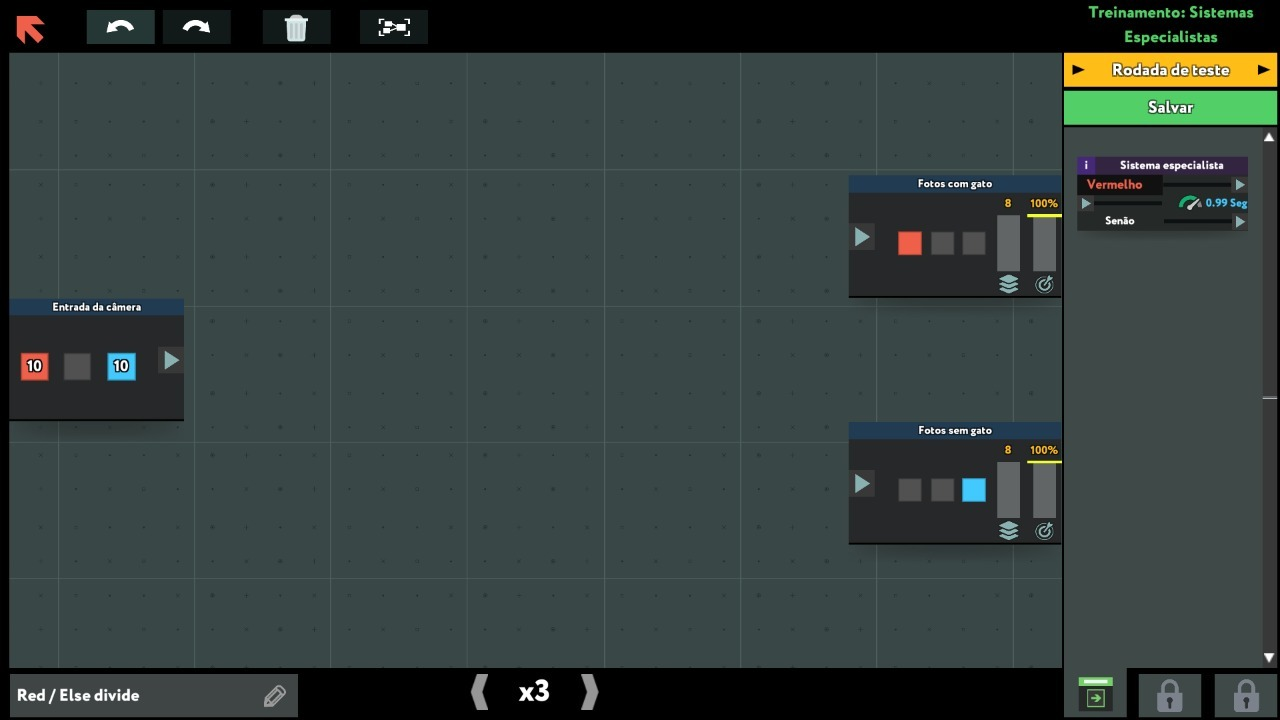
\includegraphics[width=0.9\textwidth]{fase}
    \fonte{\citeonline{while-true-learn}}
\end{figure}

\newpage

Para fazer o jogo, será necessário entender alguns componentes essenciais.

\vspace{1em}

\begin{figure}[!h]
    \centering
    \legenda[fig:componentes-da-fase]{Componentes da fase}
    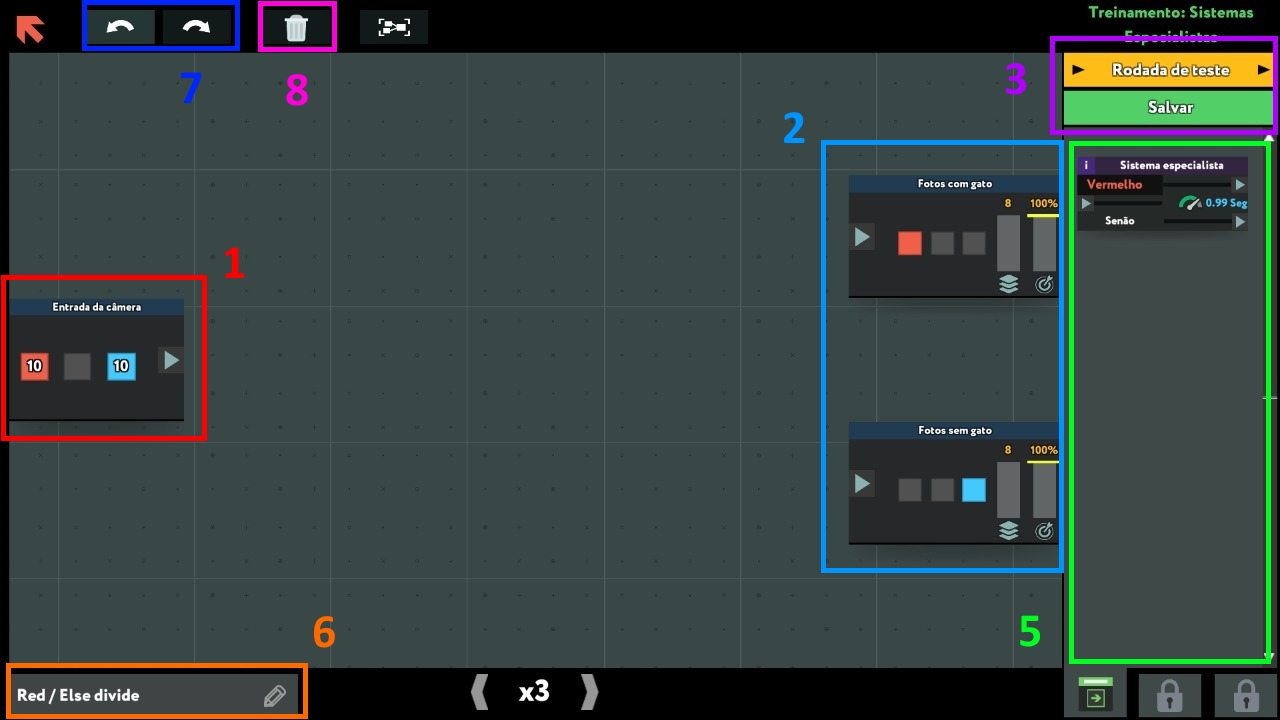
\includegraphics[width=0.9\textwidth]{componentes-da-fase}
    \fonte{\citeonline{while-true-learn}}
\end{figure}

\vspace{1em}

O componente 1 é a entrada que irá mandar um dado aleatório em seu armazenamento para a sua saída.

O componente 2 são as saídas que receberão os dados enviados para suas respectivas entradas.

O componente 3 são o botão que roda o programa e o botão que salva o esquema.

O componente 5 é onde estão guardados os nós que poderão ser arrastados para serem colocados no programa.

O componente 6 é o nome do esquema que poderá ser modificado.

O componente 7 é o botão de fazer e desfazer.

E o componente 8 é botão que deleta todos os nós utilizados.

\newpage

Também será necessário criar uma tela para o sucesso do esquema.

\begin{figure}[!h]
    \centering
    \legenda[fig:tela-de-sucesso]{Tela de sucesso}
    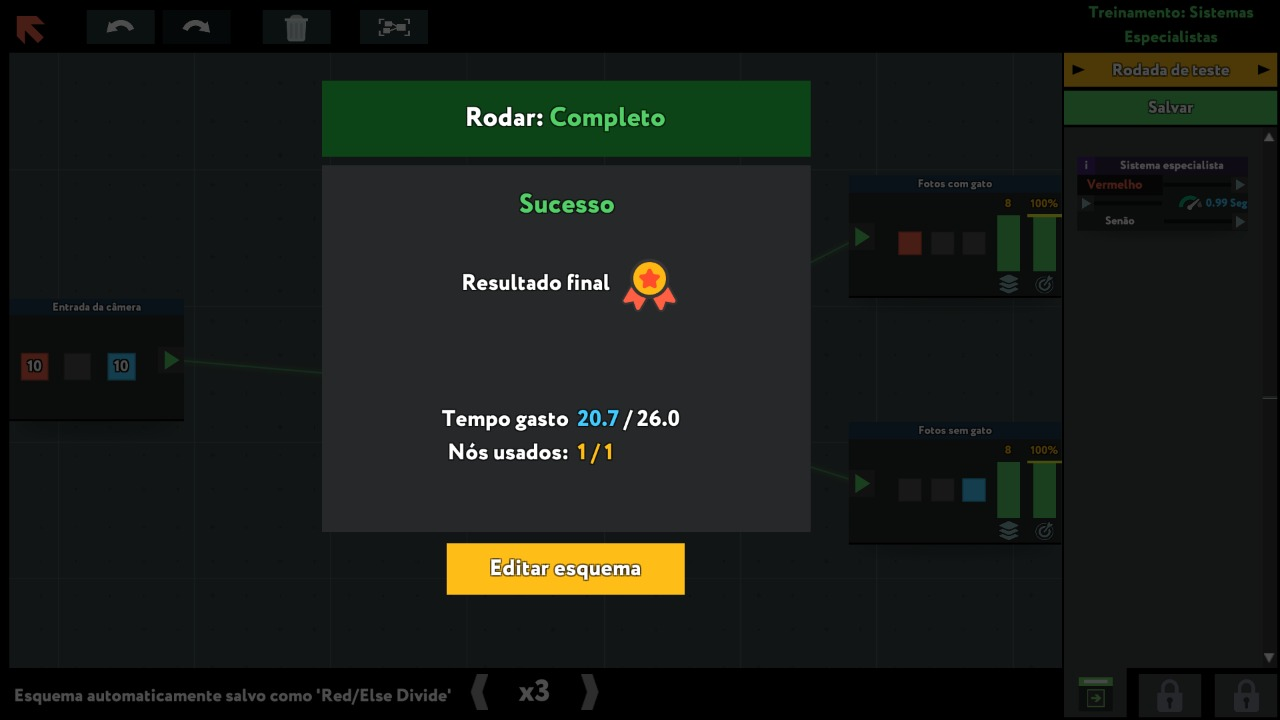
\includegraphics[width=0.9\textwidth]{sucesso}
    \fonte{\citeonline{while-true-learn}}
\end{figure}

Assim como uma tela para o fracasso do esquema.

\begin{figure}[!h]
    \centering
    \legenda[fig:tela-de-fracasso]{Tela de fracasso}
    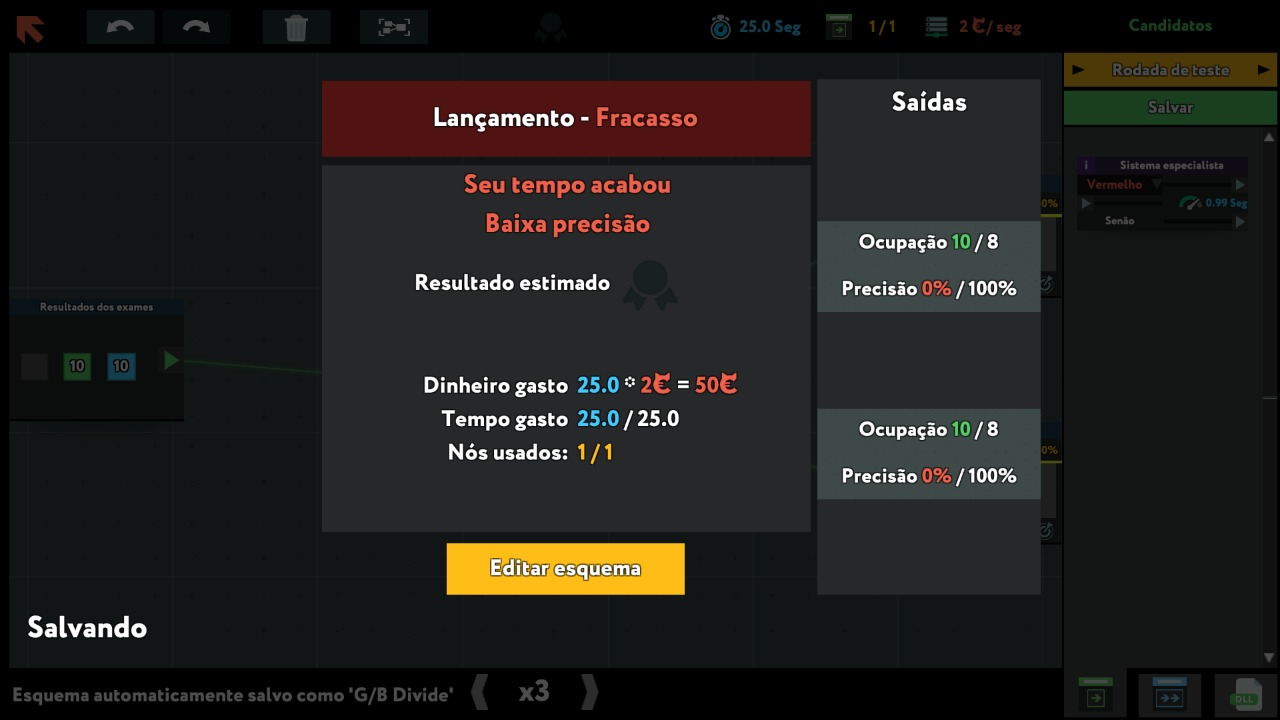
\includegraphics[width=0.9\textwidth]{fracasso}
    \fonte{\citeonline{while-true-learn}}
\end{figure}

A \autoref{fig:tela-de-fracasso} mostre a tela de fracasso de outra fase, pois na primeira fase do jogo é impossível ver uma tela de fracasso.

\newpage

Na primeira fase, ao invés de uma tela de fracasso, o jogo informa o usuário o que está fazendo de errado.

\begin{figure}[!h]
    \centering
    \legenda[fig:conectadas-incorretamente]{Se as entradas e saídas estiverem conectadas incorretamente}
    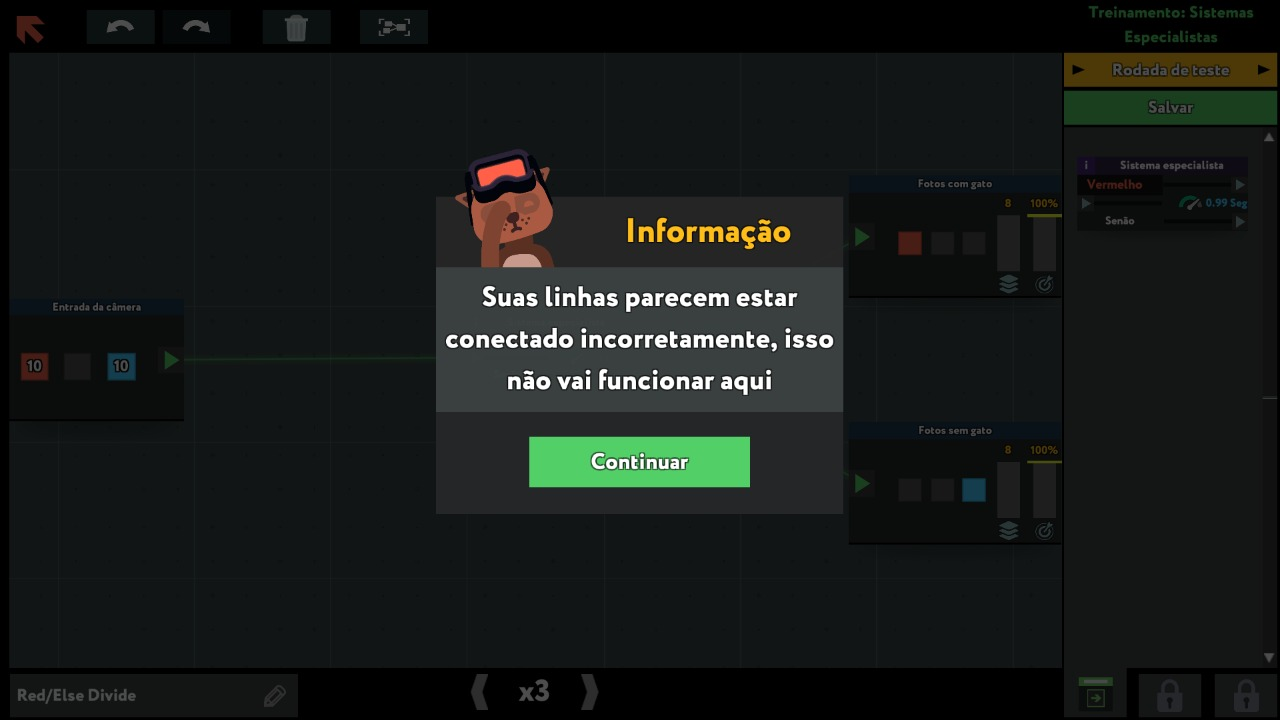
\includegraphics[width=0.9\textwidth]{conectadas-incorretamente}
    \fonte{\citeonline{while-true-learn}}
\end{figure}

\begin{figure}[!h]
    \centering
    \legenda[fig:pelo-menos-um-noh]{Se o jogador não colocar pelo menos um nó}
    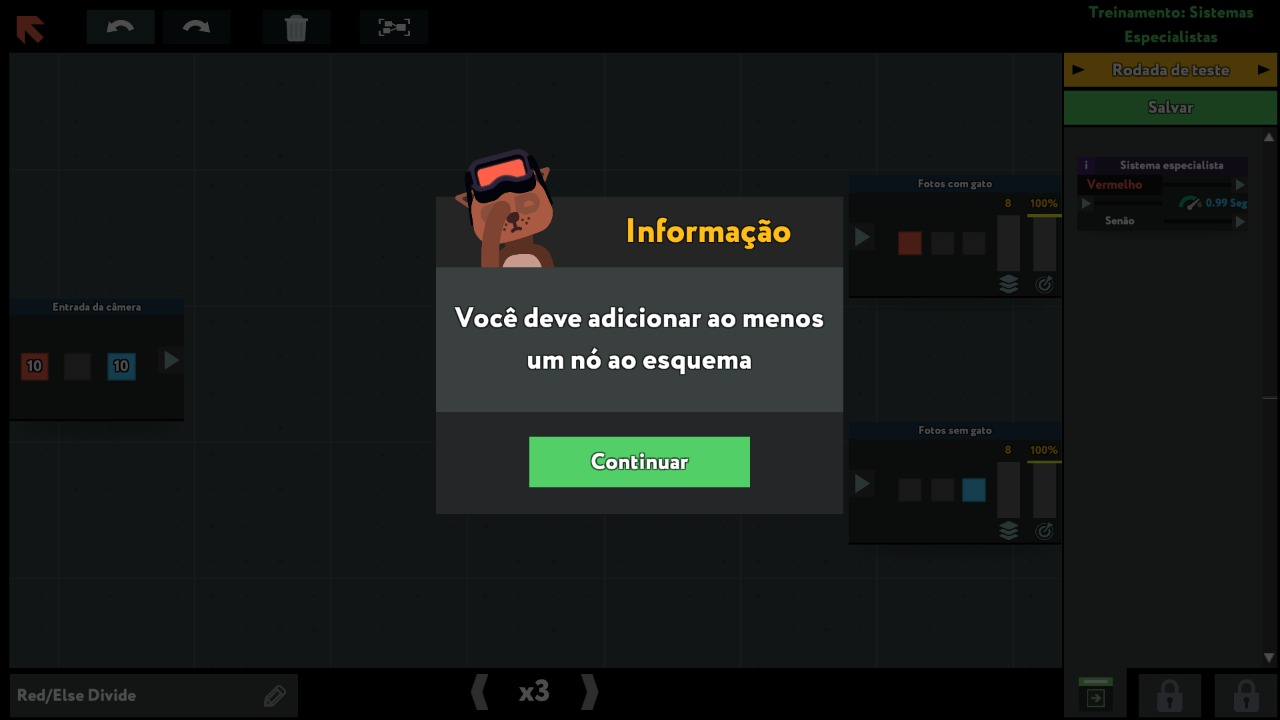
\includegraphics[width=0.9\textwidth]{pelo-menos-um-noh}
    \fonte{\citeonline{while-true-learn}}
\end{figure}
% -----------------------------------------------------------------------
% -----------------------------------------------------------------------
\chapter{Histórico do jogo}
\label{cap:historico-do-jogo}

A versão Alfa do jogo foi aberta a todos em novembro de 2017 com o modelo de "Pague o quanto quiser" para ajudar o jogo.
Em 29 de Março de 2018 foi liberado o acesso antecipado na plataforma Steam.
Em 17 de janeiro de 2019 foi lançado oficialmente na plataforma Steam.

% -----------------------------------------------------------------------
% -----------------------------------------------------------------------

% ----------------------------------------------------------
% ELEMENTOS PÓS-TEXTUAIS
% ----------------------------------------------------------
%\postextual
% ----------------------------------------------------------

% ----------------------------------------------------------
% Referências bibliográficas
% ----------------------------------------------------------
\bibliography{referencias}

\end{document}
